\documentclass{standalone}
  \usepackage{tikz}
  \begin{document}
    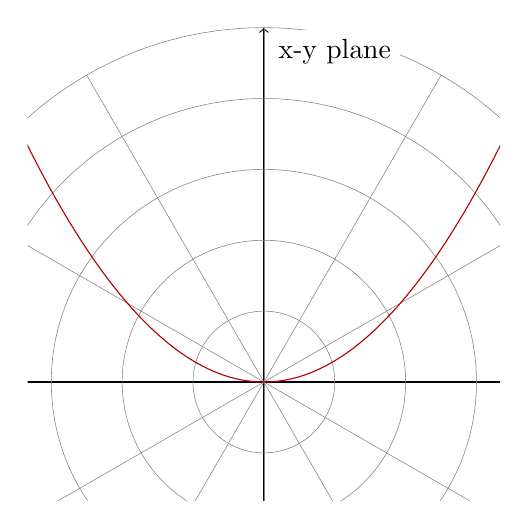
\begin{tikzpicture}[scale=3]
    \clip (-1,-0.5) rectangle (1,1.5);
    \draw[->] (-1.5,0) -- (1.5,0) node[right] {$x$};
    \draw[->] (0,-1.5) -- (0,1.5) node[above] {$y$};
    \foreach \x in {0.3,0.6,0.9,1.2,1.5}
      \draw[gray,very thin] (0,0) circle [radius =\x];
    \foreach \x in {30,60,90,120,150}
      \draw[gray,very thin] (\x:-1.5)--(\x:1.5);
      \draw[red!70!black,domain=-1.5:1.5,samples=500] plot 
          (\x, {\x*\x});
      \draw (0.3,1.4) node [fill=white]
          {x-y plane};
    \end{tikzpicture}
  \end{document}